\documentclass[letterpaper,11pt]{article}
\usepackage{tabularx}
\usepackage{amsmath}
\usepackage{graphicx}
\usepackage[margin=1in,letterpaper]{geometry}
\usepackage[final]{hyperref}
\usepackage{lineno}
\usepackage{siunitx}
\usepackage{xspace}
\usepackage{multirow}
\usepackage{enumitem}% http://ctan.org/pkg/enumitem
%%%%%%%%%%%%%%%%%%%%%%%%%%%%%%%%%%%%%%%%%%%%%%%%%%%%%%%%%%%%%%%%%%%%%%%%

\setlist[description]{labelindent=25pt,style=multiline,leftmargin=2.5cm}
\linenumbers
\newcommand{\ws}{\ensuremath{s_\mathrm{w}} \xspace}
\newcommand{\wdam}{\ensuremath{d_\mathrm{w}} \xspace}
\newcommand{\psoc}{\ensuremath{p_\soc} \xspace}
\newcommand{\soc}{\ensuremath{\mathrm{SoC}} \xspace}
\newcommand{\sob}{\ensuremath{\mathrm{SoB}} \xspace}
\newcommand{\dave}{\ensuremath{d_{\mathrm{ave}}} \xspace}
\newcommand{\dswing}{\ensuremath{d_{\mathrm{swing}}} \xspace}
\newcommand{\dphys}{\ensuremath{d_{\mathrm{phys}}} \xspace}
\newcommand{\dholy}{\ensuremath{d_{\mathrm{holy}}} \xspace}
\newcommand{\armor}{\ensuremath{a}\xspace}
\newcommand{\lvl}{\ensuremath{l}\xspace}
\newcommand{\pwf}{\ensuremath{p_{\mathrm{WF}}} \xspace}
\newcommand{\dr}{\ensuremath{DR(\%)} \xspace}
\hypersetup{
	colorlinks=true,       % false: boxed links; true: colored links
	linkcolor=blue,        % color of internal links
	citecolor=blue,        % color of links to bibliography
	filecolor=magenta,     % color of file links
	urlcolor=blue         
}
%\setlength{\parindent}{0pt} 

%%%%%%%%%%%%%%%%%%%%%%%%%%%%%%%%%%%%%%%%%%%%%%%%%%%%%%%%%%%%%%%%%%%%%%%%

\begin{document}
	
	\title{The Mathematics of Ret Paladin Rotations}
	\author{Swedge}
	\date{\today}
	\maketitle
	
	\begin{abstract}
		This document describes a formulation of ret paladin rotations in BCC by considering relative damages of different options in a paladin's rotation.
		We use this to verify the standard rotations as a function of haste, and to evaluate the optimal delays on Crusader Strike to enable imminent twists.
	\end{abstract}
	
	%%%%%%%%%%%%%%%%%%%%%%%%%%%%%%%%%%%%%%%%%%%%%%%%%%%%%%%%%%%%%%%%%%%%%%%%
	\section{Introduction}
	
	Retribution paladin in BCC relies heavily on ``seal twisting'' to increase the class's damage output.
	This technique of swinging with two active seals was an artefact of ``spell batching'' in retail BC, where as an optimisation the server processed batches of actions that would be evaluated together.
	
	In BCC, the batch size was greatly reduced, but some seals were changed to persist for a very short time after switching to another seal.
	This allows the paladin to change seals very shortly before a swing, and to have both seals active. For reasons we will cover when looking at the paladin's abilities, this results in some multiplicative damage effects over strictly additive ones, significantly increasing the paladin's damage output.
	
	In this document, we will first examine the ret paladin's abilities and the buffs we commonly utilise.
	We will then define expected damage outputs as a relative fraction of weapon damage, starting with simple situations and later taking into account more complex considerations.
	This allows us to somewhat ignore what gear the ret is using, with some notable exceptions.
	
	%%%%%%%%%%%%%%%%%%%%%%%%%%%%%%%%%%%%%%%%%%%%%%%%%%%%%%%%%%%%%%%%%%%%%%%%
	\section{Assumptions}
	We make the following assumptions that generally hold in a PvE raiding scenario:
	\begin{itemize}
		\item the ret is lvl 70
		\item the ret is in a raid group with an enhancement shaman twisting Windfury Totem with $100~\%$ uptime
		\item the ret is attacking a boss enemy at lvl 73
		\item the ret's weapon skill is maxed out at 350
		\item the ret is hit-capped, i.e. has sufficient hit rating to remove misses from the attack table
		\item the ret is hitting the target from behind, so cannot be parried
		\item the ret is \emph{not} dodge-capped at $6.5\%$, meaning there is some finite chance for their attacks, seals, and some abilities to be dodged 
	\end{itemize}
	
	%%%%%%%%%%%%%%%%%%%%%%%%%%%%%%%%%%%%%%%%%%%%%%%%%%%%%%%%%%%%%%%%%%%%%%%%
	\section{Attack Rolls}
	
	\subsection{The Melee Attack Table}
	Basic attacks in TBC are determined as a single random roll on the server.
	This means that every possible outcome for the attack is weighed together in one roll (as opposed to e.g. a multiple roll system that first evaluates the probability of an attack to
	hit or miss, and then subsequently makes a second independent roll upon a hit to evaluate critical strike chance, glancing chance etc).
	
	Each outcome of the single roll is assigned a certain precedence, such that higher precedence outcomes have the capability under certain conditions to ``push'' lower precedence outcomes off of the attack table.
	These outcomes are:
	\begin{description}
		\item[miss] the attack misses the target and is negated.
		\item[dodge] the target dodges and the attack is negated.
		\item[parry] the target parries the attack, negating the attack and hasting their autoattack timer. Parries can only occur when attacking the target from the front.
		\item[glance] when the target is three levels or more higher than the attacker, there is a chance for the attack to be a glancing blow, which deals reduced damage. The damage reduction on the attack is rolled uniformly between $15 - 35 \%$, for an average reduction of $25\%$. When the attacker is three levels lower than the target, the chance for a glancing blow to occur is $24\%$. % should move this to its own section and give formulae
		\item[block] the target blocks the attack, reducing the damage taken from the attack in accordance with the incoming damage and the target's \emph{Block Value} statistic.
		\item[crit] the attack is a critical hit, dealing a base of $200\%$ the regular damage. Critical strike damage can be modified by gear and talents.
		\item[hit] the attack is a hit, dealing regular damage.
	\end{description}
	In practical PvE scenarios, the ret is hitting the target from behind.
	As such, the block and parry outcomes are removed from the attack table.
	The miss and dodge outcomes can be reduced or eliminated entirely through appropriate gear and talents.
	In our scenario, the target enemy is three levels higher than the ret and therefore glancing blows must be accounted for in the attack table.
	Glancing blow chance cannot be reduced.
	
	\subsection{The Special Attack Table}
	Any abilities that do ``yellow'' damage are considered special attacks (e.g. paladin's crusader strike, a Shaman's Stormstrike).
	Unlike basic attacks, special attacks are calculated using multiple rolls; the first roll determines if the attack hits its target, or is avoided in some way.
	The second roll determines if the attack is a critical hit or not.
	Finally, if the damage done belongs to a non-physical magic school, e.g. holy, then the attack can be partially resisted by a boss level mob.
	Special attacks cannot be glancing blows.
	
	\section{The GCD and ICDs}
	\subsection{The Global Cooldown (GCD)}
	The Global Cooldown or GCD is a period following an ability cast (and not a swing or seal hit) where no further casts are possible.
	The base duration of the GCD is 1.5s, but it can be reduced by Spell Haste.
	Ret paladin's commonly acquire Spell Haste through the Shaman's Bloodlust ability and the Leatherworker's Drums of Battle, which together reduce the GCD to around 1.1s.
	
	The GCD is of particular importance to a ret paladin's ability to seal twist.
	In order to twist e.g. a SoC into a SoB, the SoC ability (which is typically not the seal at the start of the swing) must be cast more than a GCD before the swing timer completes such that the paladin can cast the secondary seal before the swing completes and the attack is made.
	
	We also note that the Crusader Strike ability is not a cast and does not benefit from Spell Haste, meaning the GCD following its use is \emph{always} 1.5s.
	
	\subsection{Internal Cooldowns (ICD)}
	Internal Cooldowns refer to the time period where a given spell or ability cannot proc after proccing.
	The relevant ICDs to a ret paladin are:
	\begin{itemize}
		\item Seal of Command, which has a 1s ICD to prevent it from proccing on both an autoattack and Windfury Attack on the same swing
		\item windfury attack, which has a very short ICD to prevent it from proccing on itself
	\end{itemize}

	\section{Relevant Stats}
	In this section, we'll describe the stats relevant to the damage calculations in rotations.
	The relevant stats are those that change the relative damage projections of ret actions relative to one another.
	
	A good example of this is dodge chance.
	Large parts of a twist damage sequence must survive 2-4 dodge rolls.
	By contrast, a CS must only survive one dodge roll.
	Therefore, the relative damage projection of a CS vs a twist attempt is a function of the dodge chance.
	
	\subsection{Armor}
	Armor is a stat that reduces the amount of physical damage received by a target.
	All targets have an armor value, and BCC bosses with few exceptions typically have either 6200 or 7700 armor.
	The target's level also influences the amount of damage reduction that a given level of armor will provide.
	The damage reduction formula for targets over level 60 is given as
	\begin{equation}
		\dr = \frac{100(\armor + 1)}{467.5 \lvl -22167.5}
	\end{equation}
	where \armor is the target's armor value, and \lvl is the target's level.

	High armor targets, and lower armpen gearsets, will slightly favour rotations that twist more, and higher CS delays.	
	
	
	\subsection{Spell Resistance}
	In BCC, spells that do non-physical school damage have a chance to be resisted either fully, such that the spell is nullified, and/or partially in the case of many damaging spells.
	Partial resists result in the spell's damage being resisted by either $25\%$, $50\%$, or $75\%$.
	The chance to be resisted is dependent on the level difference between the caster and the target, the caster's Spell Penetration stat, and the target's resistance to the relevant school of magic.
	
	Ret paladins seals are instances of holy damage that cannot be fully resisted, but can be partially resisted.
	Holy is not a school of magic for which spell resistance can be acquired.
	Therefore the chance for a seal to be partially resisted is therefore entirely dictated by the level difference between the caster and target.
	
	Against raid bosses, the level difference is always equal to 3.
	In this case, the probabilities for a seal to be partially resisted are given in Table \ref{tab:glancing}.
	\begin{table}[htb]
		\centering
			\begin{tabular}{r | l}
				Resistance (\%) & Probability \\
				\hline \hline
				0 & 0.82 \\
				25 & 0.13 \\
				50 & 0.04 \\
				75 & 0.01 \\
				100 & 0 \\
				\hline
			\end{tabular}
	    	\caption{Probabilities for spell partial resists against a Boss target}		
			\label{tab:glancing}
	\end{table}
	Integrating these values gives an average damage resistance against a ret paladin's seals of $6\%$.
	
	This factor will slightly diminish the relative damage of a twist attempt vs a CS.
	
	\subsection{How to handle armor and partial resists}
	These two effects apply uniformly to all instances of physical or seal damage a paladin can output.
	It's therefore sufficient to apply these damage reductions as global factors to all physical and holy damage in the rotation.
	All armor will have a scaling factor determined by the armor pen and target armor, and all seal damage will have a scaling factor of 0.94 to account for partial resists.

	\subsection{Hit Rating and Hit Chance}
	Against level 73 (or Boss level) targets, wielders of only a single weapon need a total of $9\%$ Hit Chance to never miss a target.
	Hit rating is found on gear, and increases Hit Chance.
	At level 70, 15.8 Hit Rating increases your Hit Chance by $1\%$. 
	Paladins have access to the talent \emph{Precision}, which increases the Hit Chance and Spell Hit Chance by $3~\%$.
	The Balance specialisation of the Druid class has access to the talent Improved Faerie Fire, which increases the targets chance to be hit by $3~\%$ when affected by the Faerie Fire debuff.
	In most raiding scenarios, the ret paladin must therefore acquire at least 48 Hit Rating from their gear to attain an additional $3\%$ Hit Chance in order to fully remove the chance to miss from the attack table.
	This is almost always very trivial, and so we do not need to consider miss chance in our considerations.
		
	\subsection{Expertise Rating and Expertise}
	When melee attacking a target 3 levels higher, a player has a base $6.5\%$ chance to be dodged.
	As parries can only occur when attacking the target from the front, and we attack the target from behind, parries are usually not present in our attack table.

	Each point of Expertise reduces the target's chance to dodge or parry an attack by $0.25\%$.
	Expertise Rating is found on gear.
	At level 70, 3.9 points of Expertise Rating are required to give one point of Expertise.
	As such, a player requires 26 Expertise to totally remove dodge chance from the attack table.
	
	Ret paladins do not typically take any talents that provide Expertise.
	As such, most races of paladin must acquire 102 points of Expertise Rating from their gear in order to reach 26 Expertise.
	Humans have a racial passive that provides them with 5 Expertise when using a sword or mace.
	Human rets when using the appropriate weapon only require 82 points of Expertise Rating in order to reach 26 Expertise.
	
	Because Expertise Rating is relatively scarce on gear, most paladins retain some chance to be dodged even when wearing excellent or even optimal gear.
	A non-human ret can only acquire a maximum of 95 Expertise Rating in phase two of BCC, and therefore retains a $0.5\%$ chance to be dodged.
	Due to Expertise typically being available on gear only in large increments, it is not optimal for human rets in phase two to run a gear setup that fully eliminates dodge chance.
	P3 bis loses Expertise across the board.

	As we will cover when looking at the ret paladin's abilities later in this document, Seal spells also have a chance to be dodged.
	Because of the chained nature of a paladin's damage rolls, ret paladins benefit more from Expertise than any other melee class in BCC.
	
	\subsection{Attack Power (AP)}
	Attack Power increases base melee damage per second by 1 point for every 14 Attack Power.
	When considering rotations, this stat is of note because Windfury Attacks from an enhancement Shaman's Windfury Totem have a bonus to Attack Power.
	
	The stat, however, is actually not very relevant when considering rotations, given it scales seals, attacks, and CS uniformly.
	It does become relevant when considering rotations that allow for more filler spells to be cast, but this effect should be marginal.
	
	\subsection{Critical Strike Chance}
	Critical strike chance is the chance for an attack to critical strike.
	It is relevant to evaluating rotations because of:
	\begin{itemize}
		\item the interaction between the Libram of Avengement and Judgement of Blood
		\item for basic attacks, the single-rolled nature of the attack table, which correlates crit strike with dodge
	\end{itemize}
		
	\subsection{Critical Strike Damage}
	Critical Strike Damage accounts for any improvements to the base $200\%$ critical strike damage.
	Ret paladins without exception should use the Relentless Earthstorm Diamond as their helmet's meta gem, which provides $3~\%$ increased critical damage.
	As such, a typical critical strike for a ret paladin will do $206\%$ of the base damage.
	
	As seals, attacks, and CS all benefit from the same crit strike damage bonus, this stat is only of relevance when considering Exorcism, which crits with the usual spell crit modifiers instead of melee crit.
	
	\subsection{Spellpower}
	A player's Spellpower increases the damage of some of their abilities, by a multiple of their total Spellpower multiplied by the spell's Spell Damage Coefficient (if it has one).
	Spellpower can affect all schools of magic or individual schools.
	Outside of trash sets, rets optimally do not use any gear that includes spellpower, however one of the paladin's judgement debuffs provides a flat amount of spellpower to the Holy school.
	Some of the important abilities in ret rotations have Spell Damage Coefficients, so we must include this in our calculations.
	The spell coefficients for the spells relevant to a ret paladin's rotation are provided in Table \ref{tab:spellcoefficients}.
	
	\begin{table}[htb]
		\centering
		\begin{tabular}{r | l}
			Spell & Coefficient \\
			\hline \hline
			Consecration & 0.9524 \\
			Exorcism & 0.4286 \\
			Hammer of Wrath & 0.4286 \\
			Judgement of Blood & 0.43 \\
			Seal of Command & 0.2 \\
			\hline
		\end{tabular}
		\caption{Spellpower Coefficients relevant to a ret paladin.}		
		\label{tab:spellcoefficients}
	\end{table}

	\subsection{Haste and Haste Rating}
	
	
	%%%%%%%%%%%%%%%%%%%%%%%%%%%%%%%%%%%%%%%%%%%%%%%%%%%%%%%%%%%%%%%%%%%%%%%%
	\section{Ret Abilities}
	We will now detail the most important abilities to a ret's rotation.

	\subsection{Autoattacks and Windfury Attacks}
	The largest portion of a ret's damage output comes from autoattacks and Windfury Attacks.
	As our hypothetical ret is hit-capped, misses are removed from the attack table, but they are not dodge-capped, so dodges will still be present in accordance with the ret's expertise stat.
	
	Windfury Attacks get a bonus to AP, so they are more damaging than regular attacks by a constant damage factor.
	This means that as the ret's total amount of AP goes up, the difference in the average damage between a regular attack and a windfury attack goes down.
	
	Windfury attacks caused by the max rank Windfury Totem get a bonus to attack power of 445AP, which is usually increased by $15~\%$ by taking one rank in Improved Weapon Totems talent in the Enhancement tree for a total of 511.75AP.
	This adds approximately 41.3dps to the attack, meaning that the damage added to the attack is dependent on the weapon's base speed.
	For e.g. $\ws = 3.6~\mathrm{s}$ the attack's damage is increased by approximately 131 damage.
	The formula to calculate this extra damage is given by:
	
	\begin{equation}
		d = \frac{511.75 \ws}{14}
	\end{equation}
	
	\subsection{Seals and Judgements}
		
	\subsubsection{Seal of Command (SoC)}
	This ability gives the paladin a chance to do $70\%$ of their weapon damage as holy on their attack.
	The chance is determined by the base weapon speed of the paladin's weapon, and is normalised at 7 procs per minute (PPM).
	The proc chance of SoC is therefore given by:
	
	\begin{equation}
		\psoc = \frac{7 \ws}{60}
	\end{equation}
	where \ws is the base swing speed of the paladin's weapon in seconds.
	This is the primary reason that ret paladins favour slow weapons - under no melee haste and neglecting Windfury hits, a fast-swinging weapon procs SoC on average 7 times for low damage due to the PPM normalisation, while a slow-swinging weapon procs SoC 7 times on average per minute for high damage.
	The proc chance is unchanged by haste effects, meaning that one can proc SoC well over 7 times per minute while under high haste.
	There is no limit on how many times SoC can proc in any given minute.
	
	\begin{itemize}
		\item SoC has an internal cooldown (ICD) of 1s, meaning that it cannot be procced on e.g. both melee hits in a windfury attack (but it can proc on a windfury attack if it \emph{does not} proc on the initial melee hit).
		\item SoC \emph{lingers}, meaning it persists for 400~ms after the paladin casts another seal. As such, it can be used as the first seal in a twist attempt.
		\item SoC is implemented as an attack that does Holy damage, and is subject to the basic attack table and to partial resists.
		\item It has a spell damage coefficient of 0.2 (given in \tabref{tab:spellcoefficients}).		
		\item SoC can proc Seal of Blood (See \secref{sec:sob}).		
	\end{itemize}
	
	\subsubsection{Judgement of Command}
	When the ret has SoC active, the Judgement ability will deal an amount of holy damage to the enemy, which is increased against incapacitated targets.
	Because SoC is the best seal to start a twist from, its judgement is never used in PvE content.
	As such we will not go into detail on its damage, or any related libram effects that improve SoC's judgement.
	
	\subsubsection{Seal of Blood (SoB)}
	\label{sec:sob}
 	This seal gives the paladin a $100 \%$ chance to do $35 \%$ of their weapon damage as holy on their attack, at the cost of the paladin losing health equal to $10 \%$ of the damage inflicted.
	\begin{itemize}
		\item SoB has no ICD, meaning it can proc on both hits of a swing under Windfury Attack.
		\item SoB does not linger, meaning that it can only be twisted into, and not as the first seal in a twist.
		\item SoB is implemented as an attack that deals holy damage, and is therefore subject to the attack table and to partial resists.
		\item SoB cannot proc SoC or Windfury Attack.
	\end{itemize}
 	
	\subsubsection{Judgement of Blood}
	When the ret has SoB active, the Judgement ability will deal 295 to 325 Holy damage at the cost of health equal to $33 \%$ of the damage caused.
%	The best Libram for rets in TBC is available starting in phase 1, the Libram of Avengement (see \figref{fig:loa}).
%	\begin{figure}[ht] 
%		\centering 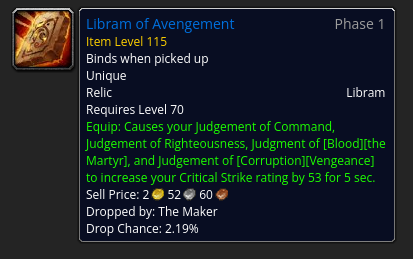
\includegraphics[width=0.44\columnwidth]{figs/libram_of_avengement.png}
%		\caption{The Libram of Avengement}
%		\label{fig:loa}
%	\end{figure}
	The Libram of Avengement causes several judgements, including Judgement of Blood, to give a buff called Justice, increasing the ret's critical strike rating by 53 for 5 seconds.
	Justice uptime varies significantly between different rotations, so should be accounted for.
	
	\subsection{Crusader Strike (CS)}
	CS is an instant cast strike that deals $110 \%$ weapon damage to the target, and refreshes all judgements on the target.
	It has a 6 second cooldown.
	
	\todo{figure out exactly how the Crusader Strike weapon damage normalisation at 3.3s actually works and how it affects the outgoing damage of the ability.}
	
	\subsection{Consecrate}
	Consecrate is an instant-cast spell that marks an area underneath the paladin, that at maximum rank deals 512 Holy damage to all enemies who are in or enter the area over 8s.

	\todo{fill out info on filler spells.}
	
	\subsection{Exorcism}
	Exorcism is an instant-cast, single-target spell that at maximum rank causes 626 to 698 Holy damage, that can only be cast on Undead or Demon targets.
	
	
	\subsection{Judgement of the Crusader}
	By default, this judgement increases the Holy damage taken by the target (by 219 at max rank).
	The ret paladin also takes 3/3 of the talent Improved Seal of the Crusader, which increases the targets chance to be critically hit \emph{by all attacks} (meaning all attacks and spells) by $3~\%$.	
	
	\subsection{Sanctity Aura}
	Without exception, ret paladin's should utilise Sanctity Aura, which gives all holy damage done by the party a $10~\%$ increase.
	This factors into the relative weight of a ret paladin's physical and holy damage, and should be considered in the rotations.
	2/2 Improved Sanctity Aura is also taken by ret paladins, which improves the amount of damage caused by targets subject to Sanctity Aura by $2~\%$.
	
	The holy damage increase from Sanctity aura does not interact with the holy damage increase from Judgement of the Crusader.
	
	%%%%%%%%%%%%%%%%%%%%%%%%%%%%%%%%%%%%%%%%%%%%%%%%%%%%%%%%%%%%%%%%%%%%%%%%

	%input{symbols}

\section{Projecting damages of individual actions}
Given all the relevant factors in a damage calculation, it is possible to express the average damage of an ability or action.
In this section, we'll derive expressions that give the average damage, or projected damage, of various actions a ret can perform.
%Now that we have detailed BCC's combat system and its facets relevant to a ret paladin's damage output, we may now turn to the task of quantifying the projected damage of various actions a ret paladin can take.
%It is of interest to be able to compare projected damage outputs of various individual actions and rotations without having to simulate entire gear sets.
%Unfortunately, many aspects of a paladin's gear directly affect the relative effectiveness of different actions and rotations.
%These effects are often small, but can be significant.
%For example:
%\begin{itemize}
%	\item the paladin's Expertise affects the chance for their attacks to be dodged. When the dodge chance is lower, swing actions that involve many segments of damage being chained together increase in relative value to ``simpler'' swings, as a dodge breaking the damage chain is less likely to occur.
%	\item the Libram of Avengement crit buff is \emph{relatively} more effective in gear sets that have low amounts of Critical Strike Chance, and therefore rotations that provide the ability to use judgement on cooldown rise in \emph{relative} value more for lower crit gear sets (though the effects are almost certainly very small)
%\end{itemize}
%It is desirable to reduce gear sets to the lowest amount of input variables possible such that these effects can be accounted for.

\subsection{Relative damages}
When figuring out what the best option for a ret's rotation, it is not always strictly necessary to include the full damage calculation.
Let us consider the case of evaluating how riding blood and command for a swing compare to one another.
Both benefit equally from any global modifiers to a paladin's damage, e.g. $2~\%$ from the Improved Sanctity Aura talent.
They also benefit equally from the $6~\%$ damage modifier to damage dealt with two-handed weapons from the Two-Handed Weapon Specialisation talent.
We therefore do not need to include these damage scaling factors when comparing riding SoC to SoB.

An example of a relevant damage factor is Sanctity Aura itself, which increases all holy damage done by $10~\%$.
If swinging SoB and SoC have a different average amounts of holy damage (spoiler: they do) then sanctity aura affects the relative worth of riding SoC vs SoB.
In this section, we will only be analysing the following actions as independent events:
\begin{itemize}
	\item autoattacks and windfury attacks
	\item seal damage, including twists
	\item crusader strike
\end{itemize}
The statistics affecting the relative damage of each of these actions are:
\begin{itemize}
	\item total attack AP, given the differing normalisations of CS and the other actions, and the bonus AP scaling on windfury attacks
	\item dodge chance
	\item armor penetration and boss armor
	\item crit strike chance (because it is correlated with dodges in autoattacks but not for seals)
	\item the base weapon speed
	\item the mean base weapon damage
\end{itemize}
With each of these variables, it is possible to evaluate the relative projected damages of each action entirely.

\subsection{Physical and Holy global scale factors}
We now define the following global scaling factors for physical and holy damage, i.e. scale factors that will apply to \emph{every instance of physical or holy damage} that is not negated by a dodge.
For physical damage:
\begin{equation}
	\fphys = 1 - \frac{\armor - \armpen + 1}{467.5 \lvl -22167.5}
\end{equation}
where \armor is the target armor, \armpen the ret's armor penetration, and \lvl the target level.
\noindent
For holy damage:
\begin{equation}
	\fholy = 0.94 \times 1.1 = 1.034
\end{equation}
where the first term is the average reduction from partial resists, and the latter term the damage bonus to holy abilities from Sanctity Aura.

\subsection{Units of damage}
Seal of Blood, Seal of Command, and Crusader Strike are all evaluated in terms of a percentage of the paladin's weapon damage.
The average weapon damage of a paladin's basic autoattack is therefore a useful metric to start with.
We first define the average weapon damage as the damage that occurs when a weapon rolls a median value on its damage range, and is a regular hit (i.e. not a crit, or a glancing blow) that is not negated (through a miss or dodge).
\begin{equation}
	\dave = \left( \bar{\wdam} + \frac{x\ws}{14} \right)
\end{equation}
where $\bar{\wdam}$ is the median damage on the weapon's damage range, $x$ is the paladin's attack power, and \ws is the paladin's weapon speed.
We note that this is not applicable to CS, which has a different scaling with attack power, but this value can be used for autoattack and seal damages.

\subsection{Correlation of attacks}
Let us first consider the damage \dauto of so-called ``white hits'', meaning a simple autoattack.
The \dave figure is useful because it allows for all results of an attack table roll to be expressed in some multiple of \dave:
\begin{equation}
	\dauto = \fphys \dave \sum_n p_{\mathrm{n}} f_{\mathrm{n}}
\end{equation}
where the sum is over the $n$ possible outcomes for the attack roll that are left on the table (e.g. crit, dodge \ldots), with each scenario having a probability to occur $p_{\mathrm{n}}$, and a damage scaling factor for its outcome of $f_{\mathrm{n}}$ (e.g. $\fcrit = 2.06$ with an activated Relentless Earthstorm Diamond meta-gem).
Giving these outcomes explicitly, we arrive at the expression:
\begin{equation}
	\dauto = \fphys \dave (\pdodge \fdodge + \pglance \fglance + \pcrit \fcrit + \phit \fhit)
\end{equation}
where \pdodge and \fdodge are the probability and damage scaling of a dodge, and the other outcomes correspond to glances, crits, and regular hits. 

This expression can be simplified first by giving $\fdodge = 0$ (as dodges are negated entirely), \fhit as simply 1, and then describing \phit as the difference of 1 and the probability of all other attack outcomes (given hit expands to take up the remainder of the attack table), or
\begin{equation}
	\phit = 1 - \pglance - \pdodge - \pcrit
\end{equation}
The expression for the projected autoattack damage then becomes:
\begin{equation}
	\dauto = \fphys \dave (\pglance \fglance + \pcrit \fcrit + (1 - \pdodge - \pglance - \pcrit))
\end{equation}
The above expression projects the expected average damage from a simple autoattack, including outcomes where the attack is negated entirely from a dodge.

We note, however, that many parts of a paladin's damage output \emph{proc subsequent instances of damage that are conditional on the result of the initial part}.
In other words, a dodged attack cannot proc anything else.
If the outcome for negated attacks is included in our standard damage unit, then damage chains get messily correlated in ways that make the calculations very difficult.

Take windfury as an example.
It's not possible to say that the expected damage under windfury is therefore just an extra $20\%$ of \dauto because the expression for \dauto includes the chance for the attacks to be dodged - and if the first attack is dodged, the windfury attack never occurs.

\subsection{Fixing this problem}
We therefore want to derive an expression for the projected physical damage of an attack \emph{independently of the chance for it to be dodged}.
This is complicated by \pdodge affecting the relative magnitudes of \phit, \pglance, and \pcrit arising from the use of a single-roll attack table.
Therefore even when deriving an expression that describes only the case when the attack is \emph{not dodged}, we still expect to see \pdodge as a relevant factor.

We therefore define \dphys as the \emph{average damage from an attack that connects with the enemy}, i.e. is not dodged.
\begin{equation}
	\dphys = \fphys \dave \frac{(\pglance \fglance + \pcrit \fcrit + (1 - \pglance - \pdodge - \pcrit)}{1 - \pdodge}
\end{equation}

Note that despite the presence of two \pdodge terms, the average damage is projected \emph{only onto scenarios in which the attack connects and is not negated}.
We also see the well-established concept of a maximum limit below 1.0 on critical hit probability, or ``crit cap'' manifest in this equation, in the form of the necessary inequality:
\begin{equation}
	\pcrit \leq (1-\pglance - \pdodge)
\end{equation}
As glance and dodge have higher \emph{precedence} than crit, it can never push them off the attack table.
As such, any crit probability above $1 - \pglance - \pdodge$ will be ignored.

\subsubsection{An Example Calculation with Windfury Attack}
To see why this formulation is useful, let us now derive the projected damage in the case of a naked windfury swing in these terms.
%The typical raiding values for the above correspond to $\pglance = 0.24$, $\fglance = 0.75$, $\fcrit = 2.06$, with a probability of proccing Windfury $\pwf = 0.2$.

To be exact, we must consider that the windfury attack has an amount of bonus attack power, that depends on the rank of the Windfury Totem and the Shaman's talents.
If the ret paladin's attack power is $x$ and the bonus attack power on the Windfury Attack is $y$, the $\dave(\mathrm{wf})$ on the Windfury attack can be expressed as a fraction of the autoattack's \dave as:
\begin{equation*}
	\begin{aligned}
		\frac{\dave(\mathrm{wf})}{\dave} &= \frac{\wdamave + \frac{(x+y)\ws}{14}}{\bar{\wdam} + \frac{x\ws}{14}} \\
		&= \frac{\wdamave + \frac{\ws x + \ws y}{14}}{\wdamave + \frac{\ws x}{14}}
	\end{aligned}
\end{equation*}
We can therefore define a scale factor
\begin{equation}
	\fwf = \frac{\wdamave + \frac{\ws x + \ws y}{14}}{\wdamave + \frac{\ws x}{14}}
\end{equation}
which is the relative damage of a Windfury hit (with bonus Windfury attack power $y$, a paladin's attack power $x$, and a weapon speed \ws) to a normal autoattack hit.

The projected damage of a naked hit with Windfury active and a non-zero \pdodge is then:
\begin{equation*}
	\begin{aligned}
		d_\mathrm{wf} &= (1 - \pdodge) \dphys + (1 - \pdodge)^2 \pwf \fwf \dphys\\
				&= \dphys\left(1 - \pdodge + \pwf\fwf(1 -\pdodge)^2\right) \\
	\end{aligned}
\end{equation*}
This equation is expressed entirely in terms of our \dphys variable, the dodge chance, and the Windfury proc chance and damage scaling factor.
With this equation, you can plug in some values for the ret's stats and determine the relative benefit of swinging with windfury up over not having it.


\subsubsection{Quick aside: single attack table weirdness}
This all has some slightly counter-intuitive effects:
\begin{itemize}
	\item Low Expertise gear sets do slightly more damage on average when they hit, do less overall damage on average from being dodged more, and benefit disproportionately from Critical Strike Chance.
	\item Low Expertise gear sets do slightly less damage on average when they hit, do more overall damage on average from being dodged less, and benefit slightly less from Critical Strike Chance than low Expertise gear sets.
\end{itemize}
Ultimately because of the construction of the single-roll attack table, this makes sense.
Crits are independent of negations like miss or dodge, so regardless of your dodge chance you will crit on average the same number of swings with a given crit chance (provided you are not near the crit cap).

We provide in \tabref{tab:wfautos} some example calculations of windfury damage for three different dodge chance scenarios, in each calculating the projected damage of a set with $10\%$ crit and one with $40\%$ crit.
For each scenario, we can see that the relative benefit of moving to a higher crit value changes as a function of the dodge chance, again due to quirks in the single-roll attack table.

\begin{table}[htb]
	\centering
%	\title{Windfury attacks w.r.t. crit and dodge chance}
	\begin{tabular}{ r | r | r | r | r | l }
		  \multicolumn{1}{c|}{}  & Dodge Chance & Crit Chance & Projected \dphys & Projected \dwf & Crit Benefit \\
		\hline \hline
		\multirow{2}{*}{Scenario 1}	 &	\multirow{2}{*}{0.065} & 0.1 & $1.049~\dave$ & $1.164~\dave$ & \multirow{2}{*}{1.324} \\
					&  & 0.4 & $1.389~\dave$ & $1.542~\dave$ & \\
		\hline
		
		\multirow{2}{*}{Scenario 2}	 &	\multirow{2}{*}{0.0325} & 0.1 & $1.048~\dave$ & $1.210~\dave$ & \multirow{2}{*}{1.314} \\
		&  & 0.4 & $1.377~\dave$ & $1.589~\dave$ & \\
		\hline
		
		\multirow{2}{*}{Scenario 3}	 &	\multirow{2}{*}{0.0} & 0.1 & $1.046~\dave$ & $1.255~\dave$ & \multirow{2}{*}{1.304} \\
		&  & 0.4 & $1.364~\dave$ & $1.637~\dave$ & \\
		\hline
		
	\end{tabular}
	\caption{How dodge chance interacts with critical strike chance.
		\dave encodes all information on the user's weapon and Attack Power, so these results hold across all gear sets.
	The projected \dphys is the average damage of a connecting attack i.e. an attack that is not dodged.
	The projected \dwf is the average damage of a swing under windfury, including the chances for the attacks to be dodged.}		
	\label{tab:wfautos}
\end{table}

Somewhat frustratingly, we cannot naively say that e.g. the P2 BiS Blood-Elf scenario with 24 Expertise and $\pdodge = 0.005$ is better than a no-Expertise scenario with $\pdodge = 0.065$ by a factor of $1.193005/1.109845 \approx 1.075$.
We can only say how the relative levels of Expertise compare \emph{as a function of Critical Strike Chance}, even if the effect is marginal in most cases.

This is also why, if you somehow manage to hit a rogue with Evasion up, it will have a very high chance of being a crit, as all the lower precedence regular hits have been pushed off the table.
In that very fringe case, you don't benefit much from a high value of critical strike chance; even low crit chance gear sets will crit if they hit.

\subsection{Seal of Command swing - no windfury}
We now turn to projecting the damage of swinging with Seal of Command active, without windfury.
We no longer have to worry about the single-rolled attack table given that special attacks use an independent roll to determine if the attack connects.
We do, on the other hand, now have to worry about the differences between holy and physical damage to properly quantify the projected damage.

Using the units of damage we have arrived at previously, the damage of a SoC proc on a regular hit is simply:
\begin{equation}
	\dsocproc(\mathrm{hit}) = \fholy \left( 0.7  \dave + \fspell (\dspell + \bspell) \right)
\end{equation}
where \fspell if the SoC spellpower coefficient of 0.2, \dspell is the ret's spellpower, and \bspell is the bonus spell power to abilities cast on the target (from abilities like JotC).
When we include the chance for regular hits and crits (and because a successful seal attack can \emph{only} hit or crit):
\begin{equation}
	\dsocproc = \dsocproc(\mathrm{hit}) \times ( \pcrit \dcrit + 1 - \pcrit)
\end{equation}
AS a reminder, the proc chance for SoC is determined by the base weapon speed \ws:
\begin{equation}
	\psoc = \frac{7 \ws}{60}
\end{equation}
When we combine this with the auto that must connect to proc the SoC, taking into account the relevant dodge chances, we find the following damage projection for a swing with SoC active:
\begin{equation*}
	\begin{aligned}
		\dsocswing =&~ (1-\pdodge) \left( \dphys + (1 - \pdodge) \psoc \dsocproc \right) \\
%		=& \dphys - \pdodge \dphys + (1-\pdodge) \psoc \dsocproc - \pdodge(1 - \pdodge) \psoc \dsocproc\\
		=&~ (1 - \pdodge) \dphys + (1 - \pdodge)^2 \psoc \dsocproc\\
	\end{aligned}
\end{equation*}

\subsection{Seal of Command swing - with windfury}
The SoC ICD means that only one melee hit can proc SoC.
If the first hit procs SoC, the second cannot, and vice-versa.
We also find two possible damage chains that can occur:
\begin{enumerate}
	\item The initial melee procs \emph{both} windfury attack and SoC.
	\item The initial melee procs \emph{only} windfury attack, which subsequently procs SoC.
\end{enumerate}
Each case results in a different number of dodge checks to be passed.
In the first case the projected damage is:
\begin{equation*}
	\begin{aligned}
		\dsocswing (1) =&~ (1-\pdodge) \dphys + (1-\pdodge)^2 \psoc\dsocproc + (1-\pdodge)^2 \pwf \fwf \dphys\\
	\end{aligned}
\end{equation*}
In the second case the projected damage is:
\begin{equation*}
	\begin{aligned}
		\dsocswing (2) =&~ (1-\pdodge) \dphys + (1-\pdodge)^2 \pwf \fwf \dphys + \pwf (1-\pdodge)^3 \psoc\dsocproc\\
	\end{aligned}
\end{equation*}
These cases are mutually exclusive. Projecting over them both we find:
\begin{equation*}
	\begin{aligned}
		\dsocswing =&~ (1-\pdodge) \dphys + (1-\pdodge)^2 \pwf \fwf \dphys \\
		&+ (1-\pdodge)^2 \psoc\dsocproc \\
		&+ (1-\psoc)(1-\pdodge)^3 \pwf \psoc \dsocproc \\
		=&~  \dphys(1 - \pdodge + \pwf\fwf(1 -\pdodge)^2) \\
		&+ (1-\pdodge)^2 (1+\pwf(1-\pdodge)(1-\psoc)) \psoc\dsocproc 
	\end{aligned}
\end{equation*}
Note that the physical damage reduces down to the same result as for a naked swing under windfury; simply put, your basic attacks don't care what seal you have active, they hit all the same. We show the SoC under windfury as a function of the weapon speed in Figure \ref{fig:soc_wf} - it is very slightly nonlinear, with the proc chance increasing under windfury less at higher weapon speeds.

\begin{figure}[ht] 
	\centering 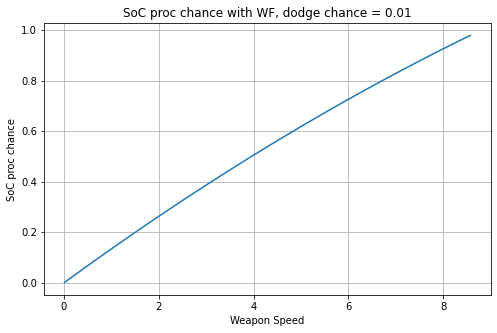
\includegraphics[width=0.84\columnwidth]{figs/wf_soc_1.png}
	\caption{SoC proc chance under windfury as a function of weapon speed, \pdodge = 0.01}
	\label{fig:soc_wf}
\end{figure}

\newpage
\subsection{Seal of Blood swing - no windfury}
Seal of Blood is a simpler ability to forecast because it has no internal ICD, meaning that there is no correlation between the SoB procs, it has no spellpower coefficient, and the proc is guaranteed.
The proc damage on a regular hit is therefore identical to the physical damage, times the $35~\%$ weapon damage scaling, and the global holy damage factor:
\begin{equation}
		\dsobproc(\mathrm{hit}) = \fholy 0.35  \dave
\end{equation}
and the corresponding damage accounting for crit chance is
\begin{equation}
	\dsobproc = \dsobproc(\mathrm{hit}) \times (\pcrit \dcrit + 1 - \pcrit)
\end{equation}
The damage for a SoB swing without windfury is therefore:
\begin{equation}
	\dsobswing = (1 - \pdodge) \dphys + (1-\pdodge)^2 \dsobproc
\end{equation}

\subsection{Seal of Blood swing - with windfury}
There is only one damage sequence for a SoB hit under windfury: the initial melee procs a SoB that must survive the standard two dodge rolls.
The windfury attack if procced must also survive two dodge rolls, and its SoB proc must survive three dodge rolls.
The damage projection for the full swing is therefore:
\begin{equation*}
	\begin{aligned}
		\dsobswing =&~ (1 - \pdodge) \dphys + (1-\pdodge)^2 \dsobproc \\
		&+ \pwf \left( (1-\pdodge)^2 \fwf \dphys + (1-\pdodge)^3 \dsobproc \right)
	\end{aligned}
\end{equation*}


%%%%%%%%%%%%%%%%%%%%%%%%%%%%%%%%%%%%%%%%%%%%%%%%%%%%%%%%%%%%%%%%%%%%%%%%
\subsection{Twist attempt - no windfury}
We now combine the information from swinging under blood and command to arrive at the damage projection for a twist attempt.
The damage sequence is as follows:
\begin{itemize}
	\item the initial melee must survive a single dodge roll, proccing a SoB that must survive two dodge rolls
	\item if command is procced, it must survive two dodge rolls, proccing a SoB that must survive three dodge rolls.
\end{itemize}
The expression is then:
\begin{equation*}
	\begin{aligned}
		\dsobswing =&~ (1 - \pdodge) \dphys + (1-\pdodge)^2 \dsobproc \\
		&+  \psoc  \left( (1-\pdodge)^2\dsocproc + (1-\pdodge)^3 \dsobproc \right)
	\end{aligned}
\end{equation*}

\subsection{Twist attempt - with windfury}
Windfury, as in the SoC swing case, introduces two possible chains for the damage procs:
\begin{enumerate}
	\item The initial melee procs both wf and SoC.
	\item the initial melee procs wf, which in turn procs SoC.
\end{enumerate}
The damage projection over the first chain is:
\begin{equation*}
	\begin{aligned}
		\dtwist (1) =&~ (1 - \pdodge) \dphys + (1-\pdodge)^2 \dsobproc \\
		&+ \psoc (1-\pdodge)^2 (\dsocproc + (1-\pdodge) \dsobproc) \\
		&+ \pwf (1-\pdodge)^2 (\fwf \dphys + (1-\pdodge)^3 \dsobproc) 
	\end{aligned}
\end{equation*}
while the damage projection over the second chain is:
\begin{equation*}
	\begin{aligned}
		\dtwist (2) =&~ (1 - \pdodge) \dphys + (1-\pdodge)^2 \dsobproc \\
		&+ \pwf (1-\pdodge)^2 (\fwf \dphys + (1-\pdodge)^3 \dsobproc) \\
		&+  \pwf \psoc (1-\pdodge)^3 (\dsocproc + (1-\pdodge) \dsobproc) \\
	\end{aligned}
\end{equation*}
Combining these two mutually exclusive chains, we find the projected damage for a windfury twist attempt:
\begin{equation*}
	\begin{aligned}
		\dtwist =&~ (1 - \pdodge) \dphys + (1-\pdodge)^2 \dsobproc \\
		&+ \psoc (1-\pdodge)^2 \left( \dsocproc + (1-\pdodge) \dsobproc \right) \\
		&+ \psoc\pwf (1-\pdodge)^2 \left(\fwf \dphys + (1-\pdodge) \dsobproc \right) \\
		&+ \pwf (1-\psoc) (1-\pdodge)^2 \left(\fwf \dphys + (1-\pdodge) \dsobproc \right) \\
		&+ \pwf(1-\psoc)(1-\pdodge)^3 \left( \dsocproc + (1-\pdodge) \dsobproc \right) \\
		=&~ (1 - \pdodge) \dphys + (1-\pdodge)^2 \dsobproc \\ 
		&+ (1-\pdodge)^2 \pwf \left( \fwf \dphys + (1 - \pdodge) \dsobproc \right) \\ 
		&+ (1-\pdodge)^2  \left( \psoc + (1-\pdodge)(1-\psoc)\pwf \right) \times \left( \dsocproc + (1-\pdodge)\dsobproc \right)
	\end{aligned}
\end{equation*}




	\appendix
	
\end{document}
